% Image wrapper: PDF table structure was not recoverable automatically.
% Requires \usepackage{graphicx}. Replace the image with tabular cells when editable text is needed.
% Caption: Table 5. It is important to emphasize that scenarios with fewer ornodynamicobstaclesaremoreeffectiveforevaluating theagent’sresponsetoredtrafficsigns,whereascrashesare appropriatelyassessedintownswithhighertrafficdensity. Generallyspeaking,BIDperformsthebestperformances acrossvariousmissions.Whenitcomestoavoidingtraffic signviolationsinthenonecase,BIDperformsnoticeably betterthanRL-Coach,whichraisestheSSR.Thisconclusion holdstrueinanormalscenarioaswell.BIDcomescloseto matchingtheexpert’sperformanceinthecrowdedscenario, outperformingRL-CoachintermsofSSRandresultingin fewercrasheswithcarsagain.Accordingtothegroundtruth, scenariothatfailedincrowdedrunsareprimarilycauseof actorsblockingup,whichcauseatimeoutduringpathfinish. Despitethis,theexpert’sperformancecanstillbeconsidered avalidupperbound. 2)Multi-sceneTransferability: Weevaluatetheresult ofBIDinincreasinglyintricaterunsthatCarlanumerous scenesprovideinthepart.WeuseCarlaofficialbenchmark measurements (Sec. IV-C1) and align the train and test settings with those used in MBI [25], as outlined in Sec. IV-A. Table II displaystheoutcomesforeverymethodthatwasoptimized usingmulti-scenedataset.Outofthe3methods,RL-Coach performstheleast,incurringmoreviolationsandresultingin anoticeablysmallerADG.APAof98\%attainedbyBIDis comparable to MBI. However, MBI has the highest ADG score (73\%),whileBIDachieves68\%.Weattributethisdifference to the fact that MBI rarely drives outside the pre-designed lane, asitisprovidedwiththeroutemapasinput.Incontrast,BID does not use an explicit route map and instead relies solely on
\begin{tabular}{c}
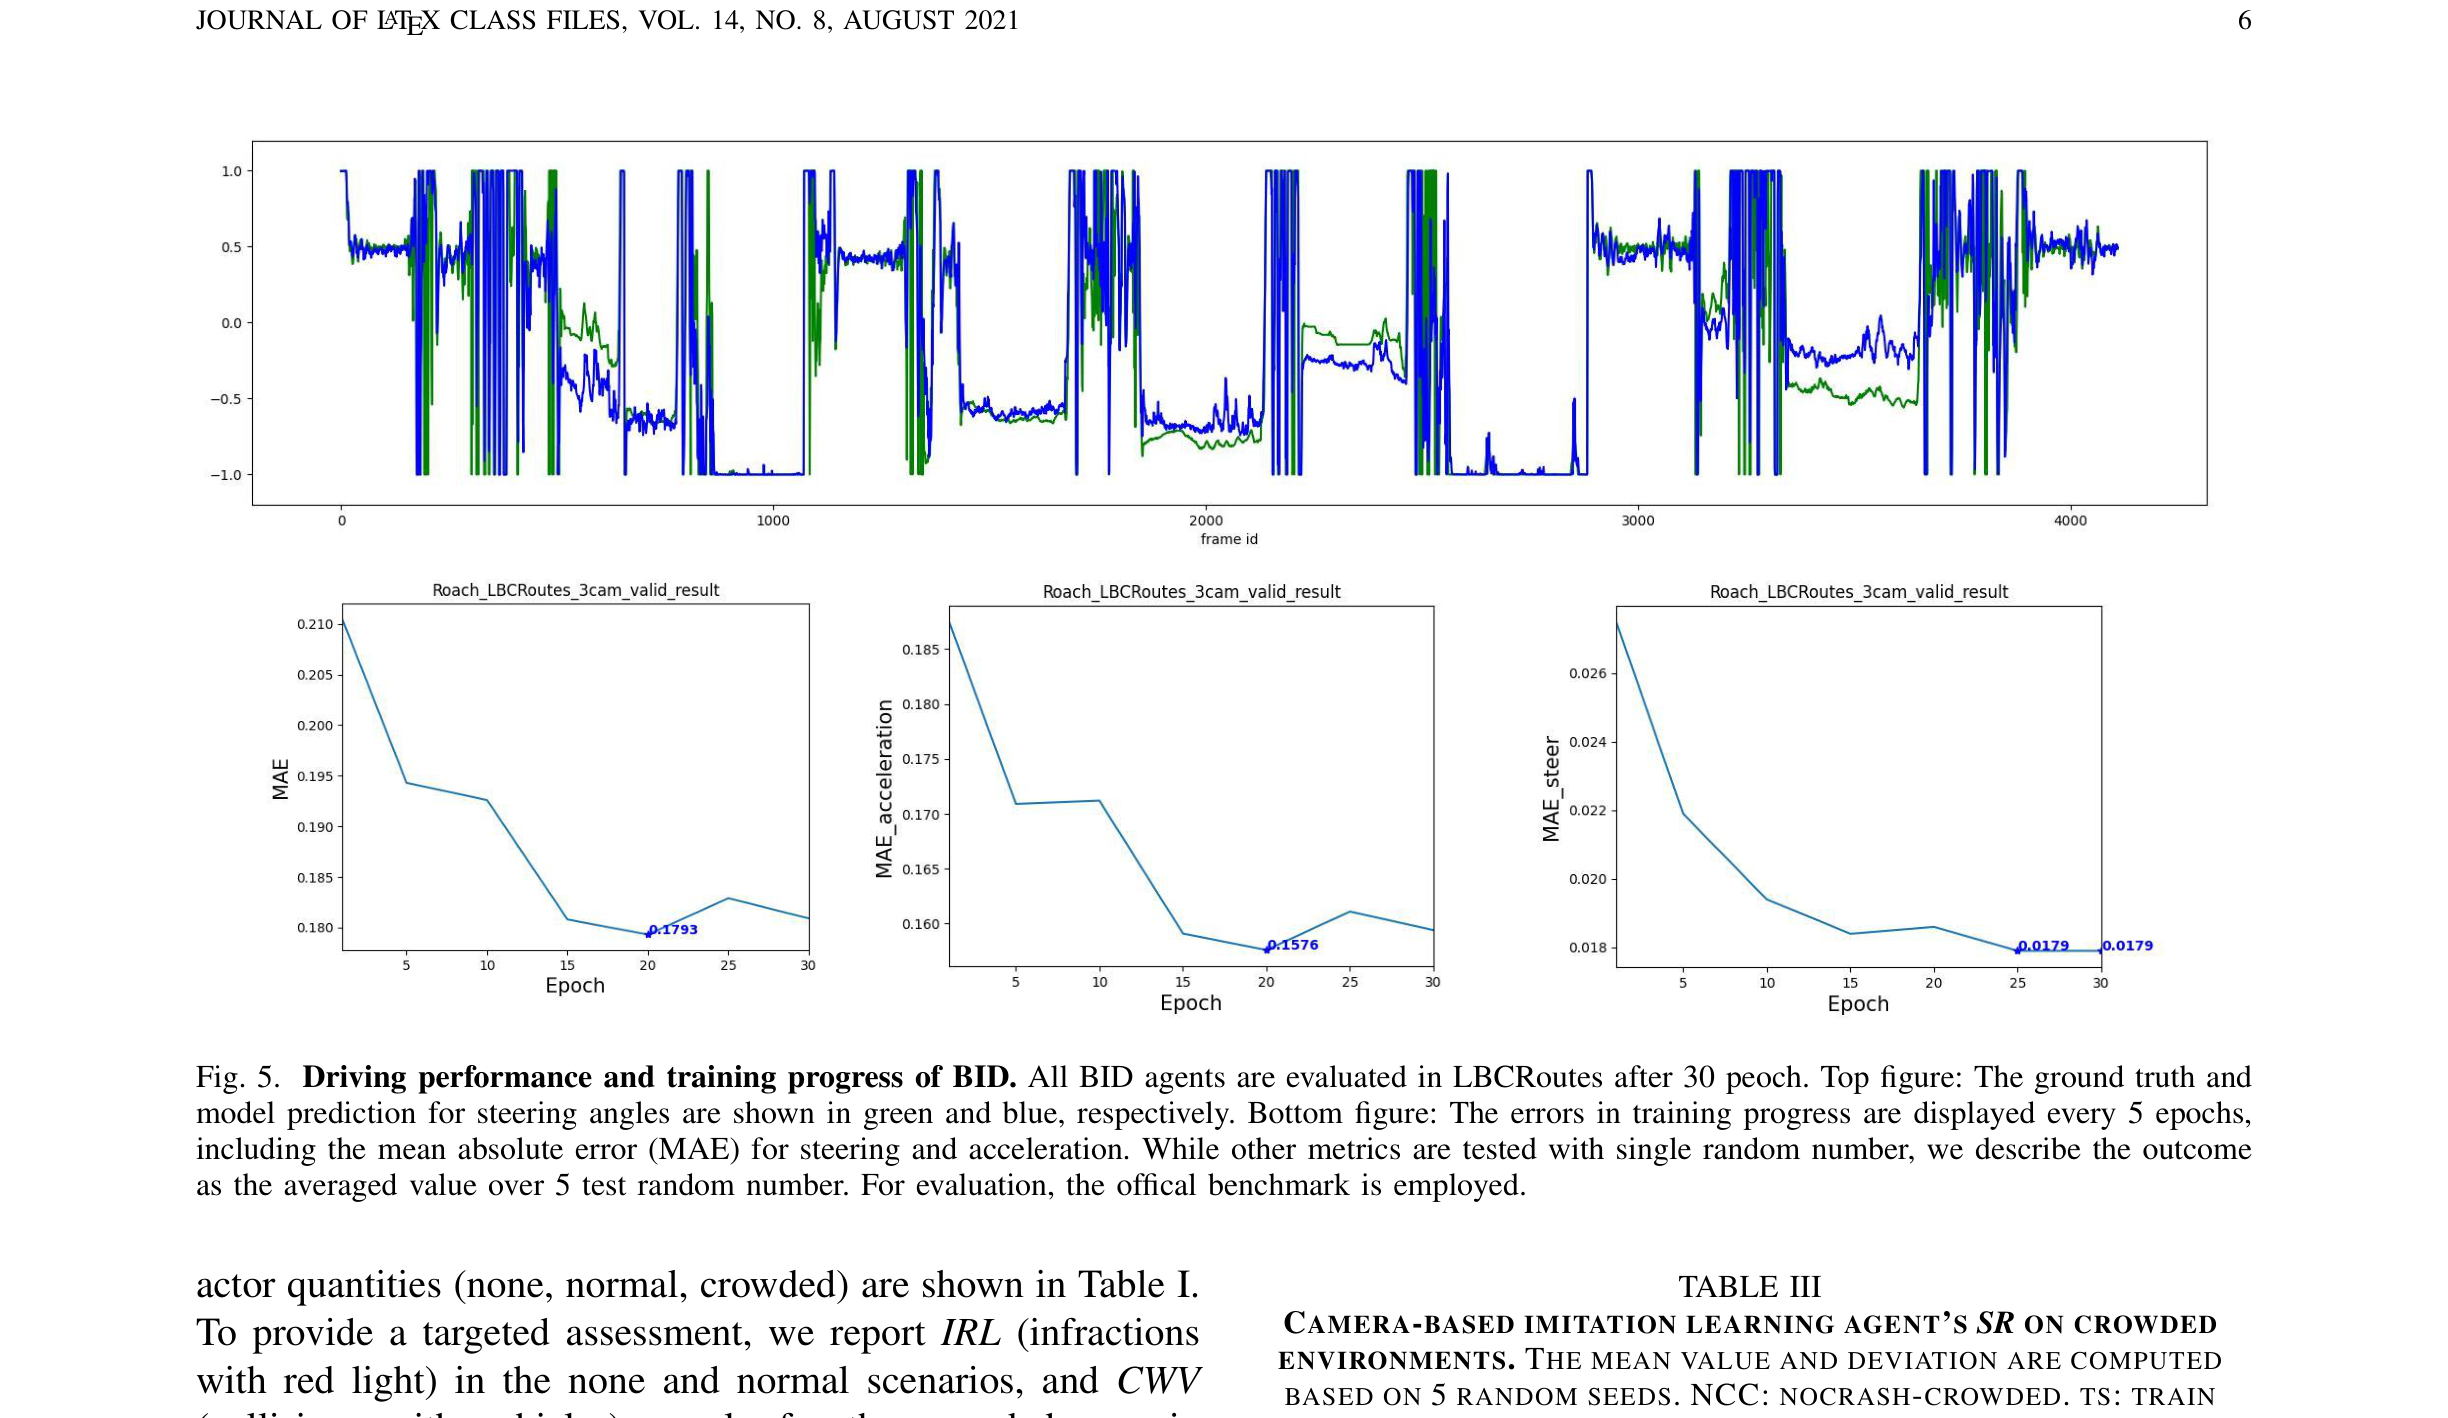
\includegraphics[width=\linewidth]{../original/Table5_p005.png}
\end{tabular}
